\documentclass[a4paper,12pt]{article}
\usepackage{amsthm}
\usepackage{amssymb}
\usepackage{amsmath}
\usepackage{hyperref}
\usepackage{xifthen}
\usepackage{xparse}
\usepackage{dsfont}
\usepackage{xcolor}
\usepackage{fullpage}
\usepackage{minted} 
\usemintedstyle{friendly} 
\usepackage{graphicx}  
\usepackage{cleveref} 
\usepackage{float}
\usepackage{caption}
\usepackage{subcaption}


% Left-right bracket
\newcommand{\lr}[1]{\left (#1\right)}

% Left-right square bracket
\newcommand{\lrs}[1]{\left [#1 \right]}

% Left-right curly bracket
\newcommand{\lrc}[1]{\left \{#1\right\}}

% Left-right absolute value
\newcommand{\lra}[1]{\left |#1\right|}

% Left-right upper value
\newcommand{\lru}[1]{\left \lceil#1\right\rceil}

% Scalar product
\newcommand{\vp}[2]{\left \langle #1 , #2 \right \rangle}


\begin{document}
\title{Assignment Title}
\author{Your Name (Your ID)}
\maketitle

\tableofcontents

\section{Introduction}
This is introduction part.

\section{Main content}
\subsection{Question 1}
\subsubsection{Code}
\begin{minted}[linenos=true, frame=single, breaklines]{python}
import numpy as np
import matplotlib.pyplot as plt


X = np.arange(10)
y = np.random.normal(0, 0.01, 10)
plt.plot(X, y)
plt.savefig(f'{output_path}q1.png', bbox_inches='tight')
\end{minted}

\subsubsection{Images}
See Fig. \ref{fig:q1} for details.
As long as the image file name remains the same, the document will be automatically recompiled to get a new PDF every time the image changes.
\begin{figure}[H]
    \centering
    \subcaptionbox{Subcaption 1}
    {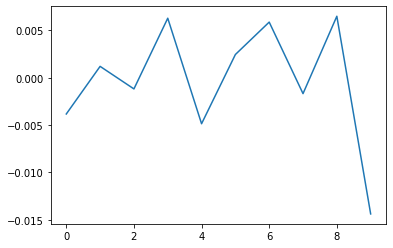
\includegraphics[width=2.5in]{../images/q1/q1.png}}
    \subcaptionbox{Subcaption 2}
    {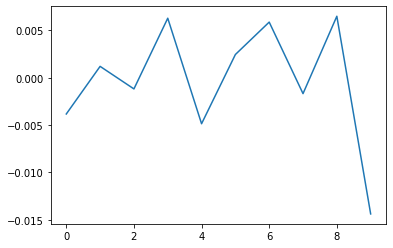
\includegraphics[width=2.5in]{../images/q1/q1.png}}
    \caption{Caption\label{fig:q1}}
\end{figure}

\subsubsection{Formulas}
\begin{align*}
    \tilde{I}\lr{x, y} &= 
    \begin{bmatrix}
        1 & 0 & t_x \\
        0 & 1 & t_y \\
        0 & 0 & 1   \\
    \end{bmatrix}
    \begin{bmatrix}
        \cos\theta & -\sin\theta & 0 \\
        \sin\theta & \cos\theta & 0 \\
        0 & 0 & 1   \\
    \end{bmatrix}
    \begin{bmatrix}
        s & 0 & 0 \\
        0 & s & 0 \\
        0 & 0 & 1 \\
    \end{bmatrix} I\lr{x,y} \\
    &= 
    \begin{bmatrix}
        s\cos\theta & -s\sin\theta & t_x \\
        s\sin\theta & s\cos\theta & t_y \\
        0 & 0 & 1   \\
    \end{bmatrix}
    \begin{bmatrix}
        x \\
        y \\
        1 \\
    \end{bmatrix} \\
    &= \begin{bmatrix}
        xs\cos\theta-ys\sin\theta+t_x \\
        xs\sin\theta+ys\cos\theta+t_y \\
        1 \\
    \end{bmatrix}.
\end{align*}

\section{Conclusion}
This is conclusion part.
\end{document}